\section{Considerações Iniciais}

Nos Capítulo X, Y, Z foram apresentadas soluções para auxiliar o engenheiro de modernização a aplicar, reutilizar e propagar refatorações no contexto da abordagem ADM e do metamodelo KDM. Além disso, no Capítulo X foi apresentado uma ferramenta, KDM-RE, que automatiza todo o processo de aplicação, reutilização e propagação de mudanças no contexto do metamodelo KDM, deixando somente sob responsabilidade do engenheiro de modernização a identificação de onde aplicar a refatoração. Desse modo, com o uso da ferramenta o engenheiro de modernização tem um ambiente totalmente integrado na IDE Eclipse, onde refatorações podem ser aplicadas e reutilizadas sem se preocupar com a propagação para outras visões/artefatos representados em um determinada instância do metamodelo KDM. 

Com o intuito de verificar se a ferramenta KDM-RE realmente proporciona tais vantagens (facilidade e eficiência) na prática, foi-se realizado um experimento ao longo deste projeto de doutorado. Esse experimento foi planejado e executado seguindo a abordagem definida por Wohlin et\change{mudar aqui}, que é composta por três principais fases: (\textit{i}) definição e planejamento, onde são especificados o contexto, as hipóteses, as variáveis, os participantes, os instrumentos e o modelo do experimento; (\textit{ii}) operação, onde ocorre a preparação e a execução do experimento com os participantes; e (\textit{iii}) análise dos dados, onde os dados coletados durante o experimento são agrupados e analisados por meio de técnicas estatísticas.

Na Seção~\ref{sec:teste_estatisticos} há uma descrição dos testes estatísticos aplicados no experimento realizado durante este projeto de doutorado. Na Seção~\ref{sec:experimento} é descrito o experimento que a ferramenta KDM-RE. Em seguida, na Seção~\ref{sec:consideracoes_finais_experimento} são comentadas as considerações finais desse capítulo.

\section{Testes Estatísticos}\label{sec:teste_estatisticos}

Wohlin et\change{mudar aqui} declaram que os experimentos têm como objetivo responder questões a respeito de um objeto de estudo. Para cada questão são definidas uma ou mais métricas a partir da qual os dados são coletados e um também um conjunto de hipóteses sobre os possíveis resultados são definidos. Esse conjunto de hipóteses é formado por:

\begin{itemize}
\item Uma \textbf{hipótese nula}: Considera que não há uma diferença significativa entre os dados obtidos ao se aplicarem os diferentes tratamentos sobre o objeto de estudo;
\item Uma ou mais \textbf{hipóteses alternativas}: Consideradam os demais possíveis resultados. Por exemplo, a hipótese alternativa 1 considera que a ferramente X é mais eficiente do que a ferramenta Y, enquanto que a hipótese alternativa 2 considerada que a ferramenta X é menos eficiente do que a ferramenta Y.
\end{itemize}

Alguns cálculos podem ser realizados sobre os dados coletados para se obter um resultado e uma das hipóteses alternativas ser aceita. Por exemplo, cálculos de média e de porcentagem podem indicar que, em determinado experimento, o tempo gasto pelos participantes para aplicar refatorações no metamodelo KDM foi menor quando a ferramenta X foi utilizada do que quando a ferramenta Y foi utiliza. Contudo, ainda se faz necessário testes estatísticos para comprovar que esse resultado é significativo, refutando assim, a hipótese nula.

No experimento apresentado nesse capítulo foram aplicado os testes estatísticos \textbf{Shapiro-Wilk} e \textbf{Paried T-Test}. Os testes estatísticos foram aplicados com o apoio da ferramenta R\change{referencia r}. Esse testes são brevemente explicados a seguir.

\subsection{Shapiro-Wilk}

O teste \textbf{Shapiro-Wilk} é aplicado para verificar se um conjunto de dados segue, ou não, uma distribuição normal, que possui graficamente o formato de um sino simétrico em relação à sua média, ver Figura~\ref{fig:shapiro_wilk}. Se o p-valor (resultado) do teste \textbf{Shapiro-Wilk} sobre um conjunto de dados for menor do que 0.05, significa que a chance dos dados seguirem uma distribuição normal é menor do que 5\%. Quando esse resultado ocorre, considera-se, estatisticamente, que os dados não seguem uma distribuição normal(wholn ref\change{colocar ref}). 

\begin{figure}[h]
	\centering
	% Requires \usepackage{graphicx}
	\caption{Representação gráfica de uma distribuição normal de dados.}
	\label{fig:shapiro_wilk}
	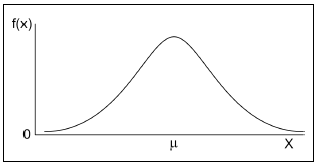
\includegraphics[scale=0.9]{images/distribuicao_normal}
	\fautor
\end{figure}

Em geral, as ferramentas de estatísticas utilizam um gráfico de propabilidade, também conhecido como \textit{Q-Q Plot} para representar graficamente a distribuição de um conjunto de dados. Nesse gráfico, quando os dados se posicionam ao redor da linha diagonal, considera-se que os dados seguem uma distribuição normal. Na Figura~\ref{fig:qq_plot_exemple} são apresentados dois exemplos de gráficos de probabilidade, um com distribuição normal e outro não normal.

\begin{figure}[h]
	\centering
	% Requires \usepackage{graphicx}
	\caption{Exemplos de gráficos de probabilidade.}
	\label{fig:qq_plot_exemple}
	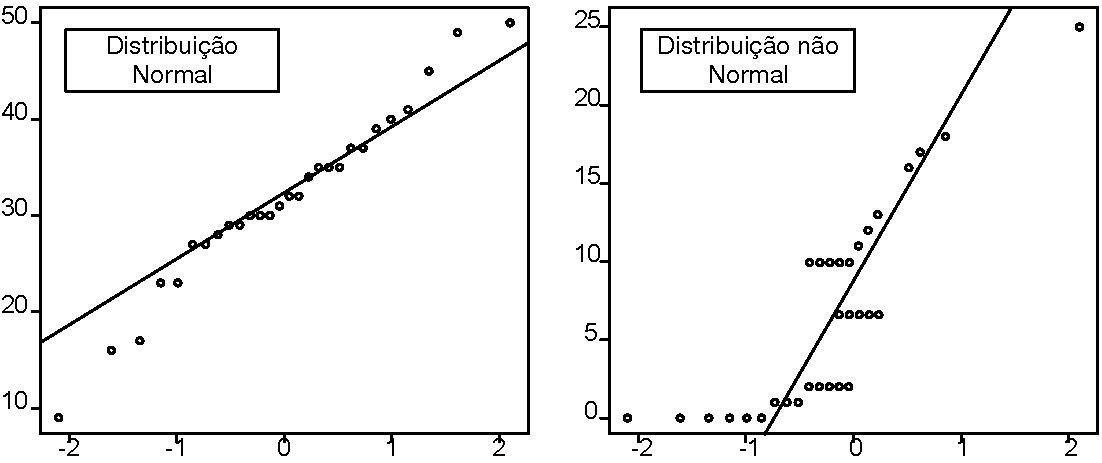
\includegraphics[scale=0.6]{images/qq_plot_exemplo}
	\fautor
\end{figure}